
\documentclass{article}
\usepackage[margin=1.0in]{geometry}
\usepackage{color}
\usepackage{caption}
\usepackage{hyperref}
\usepackage{csquotes}
\usepackage{amsmath}
\usepackage{amssymb}
\usepackage{soul}
\usepackage{changepage}
\usepackage{alg}
\usepackage{graphicx}
\graphicspath{ {./} }
\usepackage{listings}
\lstset{aboveskip=3mm, belowskip=3mm, showstringspaces=false, columns=flexible, basicstyle={\small\ttfamily}, numbers=none, breaklines=true, breakatwhitespace=true, tabsize=3}

\usepackage{newlfont}
\usepackage{program}
\catcode`\_\active

\newcommand{\define}[1]{{\sc Definition.} \textbf{#1}: }

\begin{document}
\begin{center}{\huge   Benchmarking Google Translate }\\[0.4cm]{\large  Philosophy of Computation Lab IV }\\[0.75cm]{\large  Henry Blanchette }\\[0.5cm]{\large  April 5, 2019 }\\[1.0cm]\begin{abstract}
    TODO
\end{abstract}\end{center} \section{Introduction}\section{Transcript Setup}


I selected transcript sections that reflect a variety of writing styles, including modern English, English, technical writing, storytelling, and English translated from other languages.




\vspace{1em} \noindent
Transcripts:
\begin{enumerate}
  \item[T1.] The Bible, Genesis
  \item[T2.] Melville's Moby Dick, Chapter 1
  \item[T3.] Mariam-Webster English Dictionary, definition of Abdicate
  \item[T4.] Bedau's patentsample.txt
  \item[T5.] Shakespeare's Henry IV, Part 1
\end{enumerate}

\section{Translation task}


Start with a sequence of languages $L_0, \dots, L_n$ and a transcript in $L_0$, called the \textit{original transcript.}
GT translates the $L_0$-transcript to $L_1$, and then translates the resulting $L_1$-transcript to $L_2$, and so on until the transcript has been translated to $L_n$.
At the end, there is left a $L_n$-transcript.
Then, GT translates this $L_n$-transcript back to $L_0$ - the result is the \textit{processes transcript}.
The differences between the original and processed transcripts are measured to rate GT's success at this task.
The goal of this scoring is to rate GT according to how well it preserve the meaning and grammatic structure of the original transcript.


\section{Translation Success Measure}


I rated GT's success at the task by how close the processed transcript was to the original transcript in terms of meaning and grammar. For each of these dimensions, I categorized an ranking of ordered performance classes.




\textbf{Grammar} is how properly-constructed the processed transcript is according to the rules of $L_0$ and the grammatical structure of the original transcript.
The following are the classes of grammar performance I partitioned in order of increasing success.
They are meant to be ``evenly spaced'' in the space of deviations from the exact grammar and structure of the original transcript.
\begin{align*} \begin{array}{r|l}
\text{Grammar Class} & \text{Description} \\ \hline
1 & \text{completely confused} \\
2 & \text{mostly confused} \\
3 & \text{often confused} \\
4 & \text{sparsely confused} \\
5 & \text{effectively perfect}
\end{array} \end{align*}




\textbf{Meaning} is how close the processed transcript is to the original transcript in meaning.
The following are the classes of meaning performance I partitioned in order of increasing success.
They are meant to be ``evenly spaced'' in the space of deviations from reflecting the exact meaning of the original transcript.
\begin{align*} \begin{array}{r|l}
\text{Meaning Class} & \text{Description} \\ \hline
1 & \text{irrelevant} \\
2 & \text{sparsely relevant} \\
3 & \text{often relevant} \\
4 & \text{mostly accurate} \\
5 & \text{effectively perfect} \\
\end{array} \end{align*}


\section{Predictions}


In regards to language speaker counts, I hypothesized that GT will perform better on these languages than the languages in Experiment 2 because I assume that (1) having more native speakers correlates with having more training data for GT's algorithms, and (2) having more data to train on yields a more accurate GT in the ways measured by this experiment. Assumption 1 seems very likely in general, but assumption 2 maybe depends heavily on how exactly GT works and whether it actually works well at all.





In regards to transcript style, I hypothesized that GT will perform better the more technical and less artsy the transcript. For example, I think that it will not well-maintain neither the grammatical structure nor meaning of the Shakespeare prose because it contains analogies and uncommon grammatic structures.


\section{Experiment 1: Translation Ring with Well-Documented Languages}\subsection{Language Setup}


I selected from the top 5 languages (without English) by native speaker count.   The following are the languages used in this experiment in order of decreasing native speakers count: Chinese (simplified), Spanish, Hindi, Arabic, Portuguese.




\newpage
\subsection{Experimental Design}


I ran each transcript through the following trials, where the selected languages and their order was chose randomly:
\begin{enumerate}
\item[] Trial 1: Chinese $\rightarrow$ Arabic $\rightarrow$ Spanish $\rightarrow$ Portuguese $\rightarrow$ Hindi
\item[] Trial 2: Hindi $\rightarrow$ Chinese $\rightarrow$ Portuguese $\rightarrow$ Arabic $\rightarrow$ Spanish
\item[] Trial 3: Hindi $\rightarrow$ Spanish $\rightarrow$ Arabic $\rightarrow$ Chinese $\rightarrow$ Portuguese
\item[] Trial 4: Chinese $\rightarrow$ Arabic $\rightarrow$ Spanish $\rightarrow$ Portuguese $\rightarrow$ Hindi
\item[] Trial 5: Arabic $\rightarrow$ Chinese $\rightarrow$ Portuguese $\rightarrow$ Spanish $\rightarrow$ Hindi
\end{enumerate}


\subsection{Results}
\begin{figure}[h]
\centering
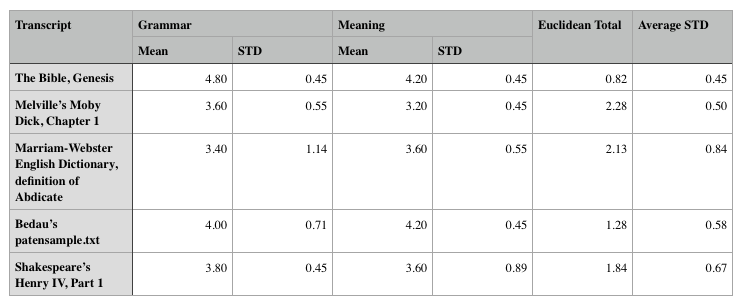
\includegraphics[width=15cm,keepaspectratio]{images/exp1-results-table.png}
\end{figure}

\begin{figure}[h]
\centering
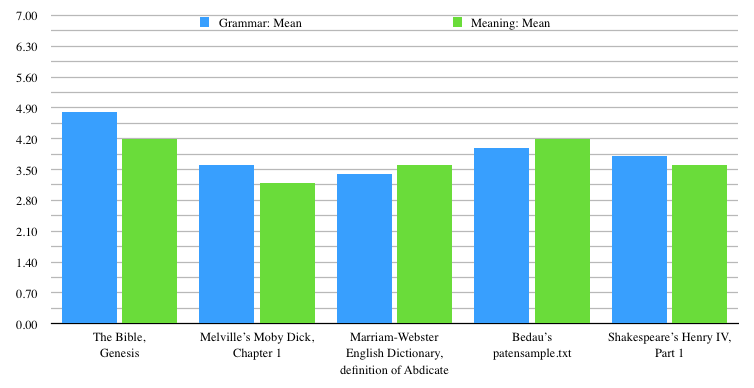
\includegraphics[width=15cm,keepaspectratio]{images/exp1-results-chart.png}
\end{figure}
\section{Experiment 2: Under-Documented Language Translation Ring}\subsection{Language Setup}


I selected from the bottom 5 languages by native speaker count that Google Translate supports . The following are the languages used in this experiment in order of decreasing native speaker count: Nepali, Sinhala, Greek, Hungarian, Zulu.




\newpage
\subsection{Experimental Design}


I ran each transcript through the following trials, where the selected languages and their order was chose randomly:




\begin{enumerate}
\item[] Trial 1: Zulu $\rightarrow$ Hungarian $\rightarrow$ Nepali $\rightarrow$ Sinhala $\rightarrow$ Greek
\item[] Trial 2: Nepali $\rightarrow$ Hungarian $\rightarrow$ Greek $\rightarrow$ Sinhala $\rightarrow$ Zulu
\item[] Trial 3: Nepali $\rightarrow$ Sinhala $\rightarrow$ Zulu $\rightarrow$ Greek $\rightarrow$ Hungarian
\item[] Trial 4: Sinhala $\rightarrow$ Greek $\rightarrow$ Nepali $\rightarrow$ Zulu $\rightarrow$ Hungarian
\item[] Trial 5: Hungarian $\rightarrow$ Greek $\rightarrow$ Sinhala $\rightarrow$ Zulu $\rightarrow$ Nepali
\end{enumerate}

\subsection{Results}
\begin{figure}[h]
\centering
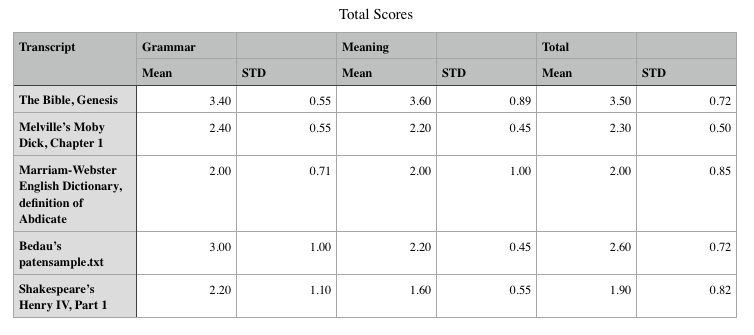
\includegraphics[width=15cm,keepaspectratio]{images/exp2-results-table.png}
\end{figure}

\begin{figure}[h]
\centering
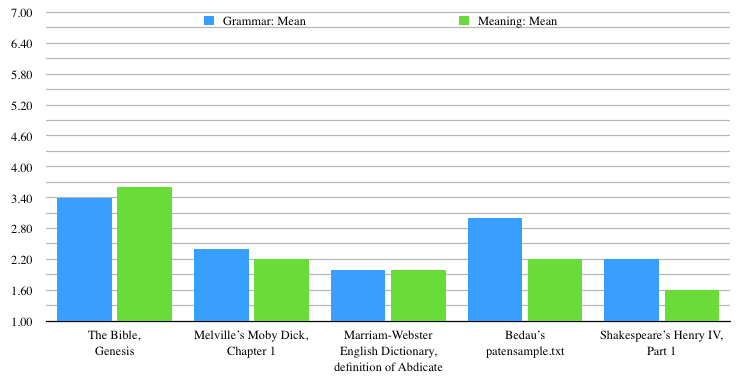
\includegraphics[width=15cm,keepaspectratio]{images/exp2-results-chart.png}
\end{figure}
\section{Analysis}\section{Conclusion}



\section*{Bibliography}
\end{document}